\begin{figure}[t]
\centering
\subfigure[Reguläres Gitter]{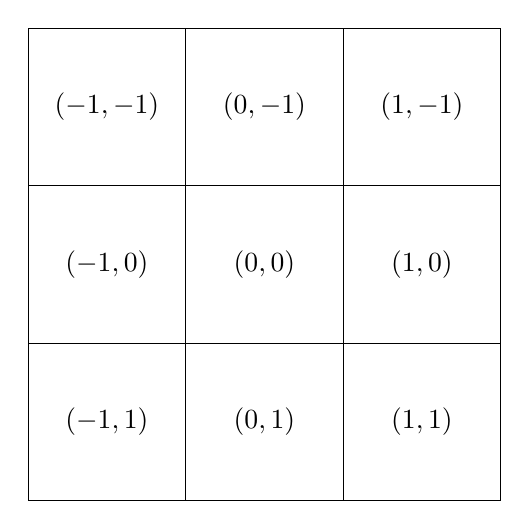
\begin{tikzpicture}
  \draw (-3, -3) rectangle (-1, -1) node[pos=0.5] {$\left(-1, 1\right)$};
  \draw (-1, -3) rectangle (1, -1)  node[pos=0.5] {$\left(0, 1\right)$};
  \draw (1, -3)  rectangle (3, -1)  node[pos=0.5] {$\left(1, 1\right)$};
  \draw (-3, -1) rectangle (-1, 1)  node[pos=0.5] {$\left(-1, 0\right)$};
  \draw (-1, -1) rectangle (1, 1)   node[pos=0.5] {$\left(0, 0\right)$};
  \draw (1, -1)  rectangle (3, 1)   node[pos=0.5] {$\left(1, 0\right)$};
  \draw (-3, 1)  rectangle (-1, 3)  node[pos=0.5] {$\left(-1, -1\right)$};
  \draw (-1, 1)  rectangle (1, 3)   node[pos=0.5] {$\left(0, -1\right)$};
  \draw (1, 1)   rectangle (3, 3)   node[pos=0.5] {$\left(1, -1\right)$};
\end{tikzpicture}
}
\hspace{1cm}
\subfigure[Graphrepräsentation]{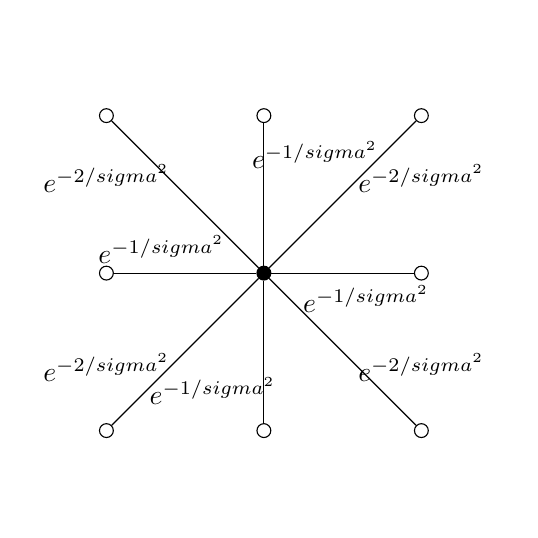
\begin{tikzpicture}
  \tikzstyle{node}=[circle,draw, minimum width=5pt, inner sep=0pt, fill=white]
  \tikzstyle{root}=[fill=black]
  \fill [white] (-3, -3) rectangle (3, 3) node {};  % Zentriere vertikal.

  \node[node] (00) at (-2, 2) {};
  \node[node] (01) at (0, 2) {};
  \node[node] (02) at (2, 2) {};
  \node[node] (10) at (-2, 0) {};
  \node[node, root] (11) at (0,0) {};
  \node[node] (12) at (2, 0) {};
  \node[node] (20) at (-2, -2) {};
  \node[node] (21) at (0, -2) {};
  \node[node] (22) at (2, -2) {};

  \path (10) edge node[shift={(-0.3, 0.3)}]  {$e^{-1/\gls{sigma}^2}$} (11);
  \path (11) edge node[shift={(0.3, -0.33)}]  {$e^{-1/\gls{sigma}^2}$} (12);
  \path (01) edge node[shift={(0.65, 0.5)}]   {$e^{-1/\gls{sigma}^2}$} (11);
  \path (11) edge node[shift={(-0.65, -0.5)}] {$e^{-1/\gls{sigma}^2}$} (21);
  \path (00) edge node[shift={(-1, 0.2)}]    {$e^{-2/\gls{sigma}^2}$} (11);
  \path (02) edge node[shift={(1, 0.2)}]     {$e^{-2/\gls{sigma}^2}$} (11);
  \path (11) edge node[shift={(1, -0.2)}]    {$e^{-2/\gls{sigma}^2}$} (22);
  \path (20) edge node[shift={(-1, -0.2)}]   {$e^{-2/\gls{sigma}^2}$} (11);
\end{tikzpicture}
}
\caption[Graphrepräsentation eines regulären Gitters]{Illustration (a) eines $3 \times 3$ großen regulären Gitters zentriert um den Punkt $\left(0, 0\right)$ und (b) dessen lokale Nachbarschaft der entsprechenden Graphrepräsentation mit einer Konnektivität von $8$ bei horizontalen \bzw{} vertikalen Kantengewichten $\exp\left(-1/\gls{sigma}^2\right) \in \gls{R}$ \bzw{} $\exp\left(-2/\gls{sigma}^2\right) \in \gls{R}$ bei den Diagonalen.}
\label{fig:gcn_review}
\end{figure}
